\section{Introducing a data visualization} \label{analysis}

To help people better understand a data visualization design, we propose a model that introduces a data visualization through constructing, which has been proven as an effective teaching method\cite{huron_constructive_2014, chapman_constructive_1988}. Thus \siwei{the conjecture is wrong here, or the logic is not correct.}, there are three questions we need to answer in our model: ``\textit{what are the basic components that compose a data visualization? }'' ,``\textit{what is the relationship between these components? }'', ``\textit{How should we deal with these relationships in our narrative?}''. At the same time, considering a large number of graphical elements \siwei{grahpical elements or graphic elements? Be consistent} employed in a data visualization design, we should eliminate the visual distraction to keep audience's focus on the target.

We propose this model based on our observation of the 375 text visualizations collected and classified in the survey made by Kucher~\cite{kucher2015text}, as well as the lessons from previous work. 

\subsection{Compositions of a Visualization}\label{compositions}
Several work focus on identifying the atomic building blocks of a visualization~\cite{mendez_ivolver:_2016, bertin1983semiology}. 
This model is the extension of previous work on taking the special requirements of presenting visual designs into consideration \siwei{what are your requirements? if you say so, please put section 4 ahead}. 
In our model, a visualization is decomposed into a hierarchical structure of three levels, including
% three levels of structure: 
visual primitives, visual units, and an advanced visualization design. 
% For example, we apply this hierarchical structure theory to 
Taking OpinionSeer~\cite{wu_opinionseer:_2010} as an example, we apply the hierarchical model and decompose it into five visual units, as shown in Figure~\ref{fig:hierarchic}. 

\textbf{A visual primitive} is one graphic element whose visual channels, such as color, width, height, are mapped to data attributes with certain visual grammar. \siwei{what is graphic element? have you defined before? I suggest you use ``atomic building blocks'' you mentioned before} For instance, a point whose size and color are encoded \siwei{are encoded to what? the sentence is broken.} is a visual primitive. Size is a visual channel, and``size indicates the importance score'' is a visual grammar. \siwei{Please define visual grammar before using an example. Further, please distinguish visual channel and visual grammar here.}


\textbf{A visual unit} is the assembly of one kind of visual primitives based on a certain construction rule \siwei{where are the construction rules come from? Cite}, as Table~\ref{tab:unit} show. 
%For the taxonomy of constructing rule, we refer the ``alignment method'' in \cite{kucher2015text} but make it more specific. 
Visual primitives of one kind can constitute different visual units by following different constructing rules \siwei{construction rule or constructing rule? Be consistent}. For example, dots can constitute scatter plot, spiral dot chart, or circle packing chart by following radial, orthogonal, or metric-based construction rules, respectively. 
\original{We are not pretending that our table includes all existing visual units, since new design is proposed constantly. }\siwei{do not say we are not pretend to do what, say we plan to do what.}
A visual unit is the smallest functional unit of a visualization. 
\original{Note that we only consider statical visualization.}\siwei{mention it in limitations} People might employ several visual primitives in an animated visualization unit.\siwei{in the first sentence, you said a visual unit is the assemble of ONE kind of... revise it.} For example, Huron et al.~\cite{huron_visual_2013} employed two visual primitives to mimic the physical process of sedimentation for visualizing data streams. 

\textbf{A visualization} can be treated as the combination of visual units. A simple visualization contains only one visual unit while an advanced one is usually the combination of multiple visual units. 
%It doesn't simply put all visual units together but constructs them based on their relationships, as described in Section 3.2.1.
% with certain connections \siwei{what is certain connections? can you give an example?} with each other, which is detailedly discussed in section 3.1.2.\siwei{where is section 3.1.2?}

\begin{figure}
 \centering % avoid the use of \begin{center}...\end{center} and use \centering instead (more compact)
 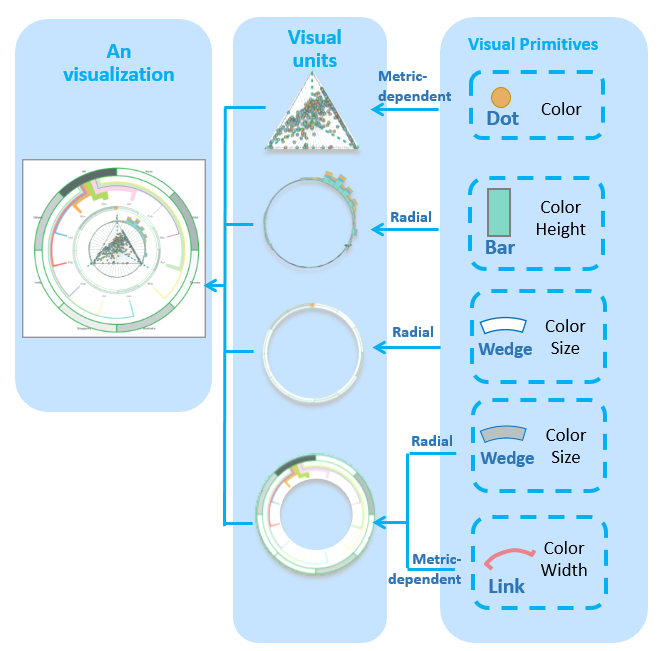
\includegraphics[width=\columnwidth]{hierarchic}
 \caption{An example of the hierarchical structure of a visualization, Opinion Seer\cite{wu_opinionseer:_2010}}
 \label{fig:hierarchic}
\end{figure}

%\begin{figure}
%\begin{minipage}{\columnwidth}
% \centering % avoid the use of \begin{center}...\end{center} and use \centering instead (more compact)
% 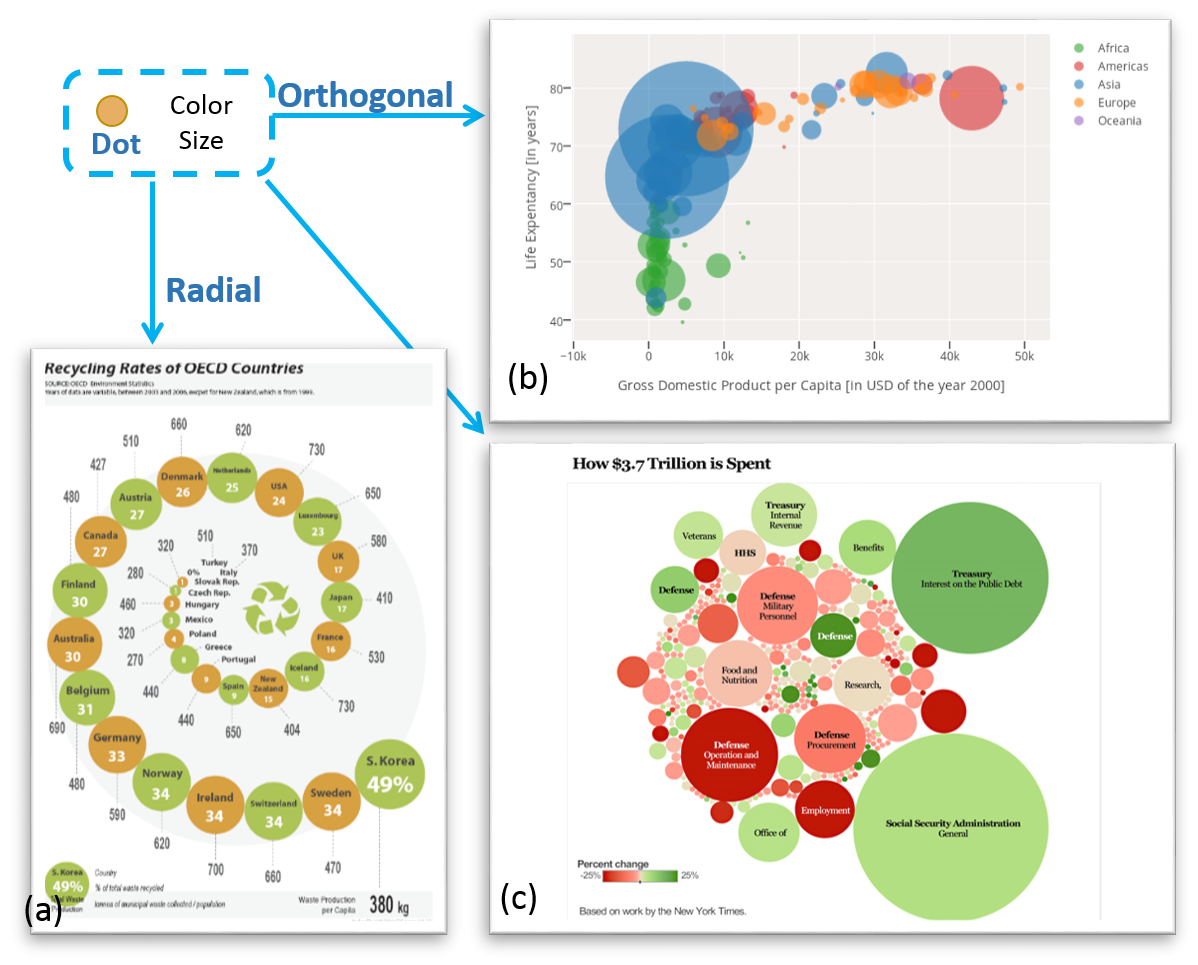
\includegraphics[width=\columnwidth]{assemble}
%\caption[assemble]
%{
%A dot, whose color and size are encoded, can assemble 
%(a) a dot spiral chart
%\protect\footnotemark{}
%    , (b)a dot packing chart
%  \footnotemark{}
%  , and (c)a bubble chart
%  \footnotemark{}
%   by following different construction rules.
%}
%\end{minipage}
%\label{fig:hierarchic}
%\end{figure}
%\footnotetext{https://www.pinterest.com/pin/16536723602037537/}
%\footnotetext{https://plot.ly/~etpinard/84.embed}
%\footnotetext{https://bl.ocks.org/mbostock/4063269}

%\begin{table*}[tb]
%  \caption{A taxonomy of visual units.\notsure{How to avoid the name ambiguities}}
%  \label{tab:unit}
%  \small
%  \centering
%  \begin{tabular}{|p{1.2cm}|p{1.2cm}|p{1.2cm}|p{1.2cm}|p{1.2cm}|p{1.2cm}|p{1.2cm}|p{1.2cm}|p{1.2cm}|}
%  \toprule
%   \textbf{} &\multicolumn{2}{|c|}{Polar Coordinates} &\multicolumn{3}{|c|}{Orthogonal Coordinates}&\multicolumn{3}{|c|}{Metric Dependent}   \\ 
%  \midrule
%  
% \textbf{} &\textbf{Radial} &\textbf{Spiral} &\textbf{Orthogonal} & \textbf{Parallel Align}&\textbf{Map}&\textbf{Cluster}&\textbf{Force-direct}&\textbf{Others}   \\ 
%  \midrule
%  \textbf{Dot} &    &Spiral Dot Chart&Scatter Plot, Bubble Chart & Dot Plot & Bubble Map &  Circle packing    &TopicPanorama\cite{7042494}  &    \\
%  \midrule
%  \textbf{Line}&  Radar Chart   &  Spiral Plot    &Node-link Diagram, Line Chart & Parallel Coordinates, Arc Diagram &    &   &     & \\ 
%  \midrule
%   \textbf{Flow}&  Chord Diagram   &    & &Parallel Sets, Sankey Diagram & 
%   Flow Map  &   &   &\\
%  \midrule
%  \textbf{Area}&    &Area Spiral Chart &Stream Graph &  & & &   &\\ 
%  \midrule
%  \textbf{Bar}&      Radial Bar Chart & Spiral Bar Chart  & Candlestick Chart & Bar Chart  &    &    &    &\\
%  \midrule
%  \textbf{Cell}& Sunburst Diagram  &    & Matrix, Tree Map &     & & &   &\\
%  \midrule
%  \textbf{Wedge}& Pie Chart, Donut Chart &  &   &   &  &    &   &\\
%  \midrule
%  \textbf{Text}&    &Parallel Tag Cloud \cite{collins2009parallel} &    &  Sentence Tree  &     &Word Cloud  &   &    \\
%  %\midrule
% % \textbf{Image}& & &Heatmap Matrix &Heatmap &\\
%  \bottomrule
%  
%  \end{tabular}
%  \vspace{1mm}
%\end{table*}

\begin{table}[tb]
  \caption{A taxonomy of visual units.\notsure{How to avoid the name ambiguities}\siwei{Use citation to avoid ambiguity. Note that the sum of column width should be around 7cm. I have changed it.}}
  \label{tab:unit}
  \small
  \centering
  \begin{tabular}{p{0.8cm}|p{2.0cm}|p{2.0cm}|p{2.0cm}}
  \toprule
%  \textbf{} &\multicolumn{2}{|c|}{\textbf{Absolute Position}} &\textbf{Relative Position}   \\ 
%  \midrule
 \textbf{} &\textbf{Radial} &\textbf{Orthogonal, Align, Map} &\textbf{Metric-based}   \\ 
  \midrule
  \textbf{Dot} &Spiral&Dot Chart, Scatter Plot, Bubble Chart, Bubble Map &Circle packing, TopicPanorama\cite{7042494}\\
  \midrule
  \textbf{Line}&  Radar Chart, Spiral Plot    &Line Chart, Parallel Coordinates, Arc Diagram &  Force-directed Node-link graph   \\ 
  \midrule
   \textbf{Flow}&  Chord Diagram   &Parallel Sets, Sankey Diagram, 
   Flow Map  & \\
  \midrule
  \textbf{Area}&  Area Spiral Chart &Stream Graph &  \\ 
  \midrule
  \textbf{Bar}&      Radial Bar Chart,Spiral Bar Chart  & Candlestick Chart, Bar Chart  &   \\
  \midrule
  \textbf{Cell}& Sunburst Diagram  &Matrix, Tree Map &  \\
  \midrule
  \textbf{Wedge}& Pie Chart, Donut Chart &  &  \\
  \midrule
  \textbf{Text}&    &  Sentence Tree  & Word Cloud \\
  %\midrule
 % \textbf{Image}& & &Heatmap Matrix &Heatmap &\\
  \bottomrule
  
  \end{tabular}
  \vspace{1mm}
\end{table}

\subsection{Relationships Between Compositions}
\label{relationship}
We first describe the relationship between conceptual compositions, then offer suggestion for narrative sequence based on these relationships. Notice that we skip the relationship between visual primitives since there is only one kind of visual primitives in a visual unit. \siwei{it is not correct. you mentioned a visual unit may contains multiple visual primitives.}

\subsubsection{Relationships Between Visual Units}
A visualization can be specified as the combination of several visual units. 
% Through observing the approaches people apply to design new visualizations, 
We go through all the text visualizations collected in Kucher and Kerren's survey~\cite{kucher2015text}, and define four types of relationships that commonly exist between visual units: irrelevance, sharing, enhancement, and dependency. 

\textbf{Irrelevance} is a bi-directional relation meaning two visual units are independent and do not share any visual channel.
For example, 2 donut charts, Figure~\ref{fig:relationship}(a) and Figure~\ref{fig:relationship}(b), are applied to illustrate the distribution of age and gender groups respectively in a population. They are put together in Figure~\ref{fig:relationship}(c) just for space-efficiency and there is no correlation between these two charts. 

\textbf{Sharing} refers to that two visual units share some visual grammars and it is a bi-directional relationship. 
For example, a line chart, Figure~\ref{fig:relationship}(d), indicates the temperature over a time period, and a bar chart, Figure~\ref{fig:relationship}(d), indicates the precipitation over a time period. They are put together in Figure~\ref{fig:relationship}(e) and they share the same visual grammar of horizontal position.  
%\siwei{what is the difference between visual grammar and visual channel? why horizontal position is visual grammar rather than visual channel?}
%\notsure{According to our survey, color and position are the most commonly shared visual encodings, which might be the result that color and position usually encoded with simple while crucial information. }


\textbf{Enhancement} is a one-way relationship. If one visual unit ``A'' is the enhancement of another visual unit ``B'', it means that ``A'' is imported into ``B'', replaces some graphical elements of ``B'', thus enables the representation of some data attributes that ``B'' alone fails to convey. Suppose there are 5 types of area in a park. A bar chart, Figure~\ref{fig:relationship}(h), illustrates their average price per unit area, a chord diagram, Figure~\ref{fig:relationship}(g), illustrates how passengers travel through each area. In Figure~\ref{fig:relationship}(i), the bar chart takes the place of node segments, which has the same height, in a chord diagram, resulting in a novel and informative visualization.
 
Enhancement widely exist in the advanced visualization design, such as the heat map mapped upon the streams in a theme river~\cite{wu_opinionflow:_2014}  and usage of glyphs to enhance the meaning of nodes in a multidimensional scaling plot~\cite{chen_peakvizor:_2016}. 

\textbf{Dependence} is a one-way relationship. If one visual unit ``A'' is dependent on ``B'', it means that ``A'' reveal some information that results from the visualization of ``B''. For example, a multiple dimensional scaling (MSD) map, Figure~\ref{fig:relationship}(j), shows the similarity between each restaurant in a city. A contour map, Figure~\ref{fig:relationship}(h), is then added to the MSD map to \notsure{show the most common type of restaurants, which information can hardly be obtained from the dataset but quite evident from the MSD map}, as in Figure~\ref{fig:relationship}(i).The biggest difference between "\textbf{enhancement}" and "\textbf{dependence}" is that 1) \textbf{enhancement} still illustrate the data attributes in the dataset, while \textbf{dependency} reveals the new knowledge we obtain from adopting a previous visualization to the dataset; 2) \textbf{enhancement} replace original graphical elements of other visual design while \textbf{dependence} adds new graphical elements.

A proper narrative sequence of visual units should take the relationships between them into consideration. For irrelevance, it doesn't matter whether these two visual units are explained sequentially. For sharing, these two visual units should be explained one after another. Since sharing is bidirectional, it doesn't matter which one is explained first. For dependency and enhancement, which are unidirectional, the two visual units should be explained sequentially in a specific order. 
 Thus, we display the correlations between units in a tree diagram where a child node is the enhancement/dependence of its parent node and sibling nodes have sharing. A proper narrative sequence can be obtained by running a deep first search on this tree diagram. 

%\subsubsection{Relationships Between Visual Primitives}
%%\siwei{There are some notes: 1. do not mention usually has 1 or 2 primitives. it is flawed. 2. Candlestick chart and error bar are quite similar expect their context. why one has no dependency and the other has logical dependency? 3. do not use two ``such as'' in one sentence.}
%%The inner relationship between visual primitives is relatively simple.
%%A visual unit usually has 1 or 2 visual primitives. 
%%
%%\notsure{
%The relationship between two visual primitives of one visual unit are usually self-evident. One primitive either has no dependency on the other one, such as the bar and line in \textit{Candlestick Chart}, or has high and evident dependency.  This dependency can be logical, such as the line and bar in \textit{error bar chart}, or spacial, such as the node segment and arc in \textit{chord diagram}, or temporal, such as the stream and dot in \cite{liu_online_2016}


\begin{figure}[tb]
 \centering % avoid the use of \begin{center}...\end{center} and use \centering instead (more compact)
 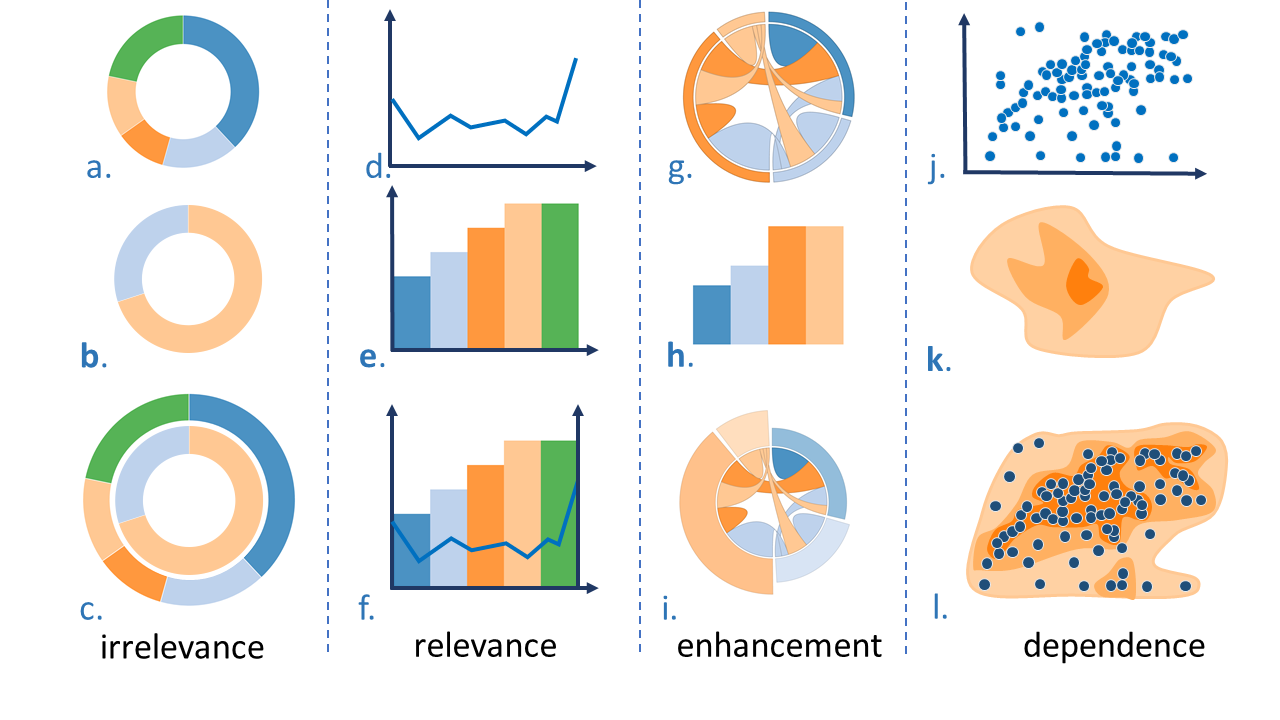
\includegraphics[width=\columnwidth]{unit_relationship}
 \caption{Illustration of the 4 types of relationship between visual units}
 \label{fig:relationship}
\end{figure}

\subsubsection{Relationships Between Visual Channels}
For a visual primitive, different channels are encoded with different data attribute. Thus, they are usually separated and have no logic dependency upon others. It's hard to determine a narrative sequence from their inner logical dependency. 

Therefore, we define two metrics to order the explaining of visual channels: \textbf{the complexity of their encoded information} and \textbf{saliency of their visual appearance}.

First, the order of decreasing visual saliency can facilitate graphical perception~\cite{cleveland_graphical_1984}. Even though different channels have intrinsically different perceptual salience and channel with high salience will suppress the expression of other, such salience strength can be influenced in a task-dependent manner ~\cite{nothdurft_salience_2000}. By introducing the channel with high saliency first, we remove it from the task list in our mind~\cite{itti2001computational}, decrease its saliency and give other channels more chance to attract the limited human attention. 

Second, the order of increasing complexity leads to an effective learning process. “Easy to difficult” practice has been long used and confirmed to be effective for learning new tasks~\cite{bliss_effects_1992}.
 
The visual saliency of different channels is relatively constant and  well defined ~\cite{munzner_visualization_2014,cleveland_graphical_1984}, while their information complexity varies in different designs. Thus, an effective narrative sequence is a trade-off between these two metrics. 

%\subsubsection{Non-linear Sequence}
%So far, all the narrative explanation we discussed is linear. However, reading a lengthy, extremely detailed instruction maybe tedious. A good narrative explanation should include non-linear design, allowing users to skip uninterested parts, go back to previous information and freely switch between different parts. Also, users should be allowed the flexibility to choose explanations at different levels of details. 

\subsection{Attention Orientation}
To keep audiences focusing on the target object, it is necessary to identify visual distractions so that measurements can be taken to avoid them. 
We identify two kinds of visual distractions: the one from context and the one from sibling channels, which refer to the visual channels belonging to the same visual primitives. 

\subsubsection{Visual distraction from the context}
This kind of distraction has been widely discussed in the field of object detection and human visual attention ~\cite{nothdurft_salience_2000, standage_modelling_2005}. Its intensity is mainly  determined by spatial distance and appearance similarity ~\cite{wolfe_guided_1994}. 
Focus + Context, which might be the most popular techniques for this problem, make uneven use of graphic resources to discriminate focus from their context. At the same time, adding dynamic changes to focus elements has also been demonstrated as effective under various conditions\cite{waldner_attractive_2014}. We support easy implementation of these techniques in our system. 

\subsubsection{Visual distraction from sibling channels}
A visual primitive usually has more than one visual channels. Thus, when recognizing one primitive, the channels with high visual saliency can significantly influence the expression of other channels. For example, color can be a strong noise when the focus is supposed to be the shape. By applying animated transition and revealing only one channel at a time, as demonstrated in \notsure{Fig1, the second line}, we are able to reduce such distraction.


